


%opening

\section{The Traditional PID Efficiency Study and MARATHON PID Difficulty}
Each arm of the HRS has two particle identification: Gas Cherenkov and Lead Glass calorimeter. Compare to the other hadrons, both of these two detectors are much more sensitive to the electrons and their PID performance is independent. In the analysis, we use these two features by applying a cut on the calibrated Cherenkov ADC sum signals and calorimeter energy (or E/P) signals to distinguish the electrons and not only that these two features can also provide us a way to check the efficiency of these two PID cuts. The tradition way \cite{pid_eff} to check the PID cut efficiency is to apply a tight cut on one of the PID detectors to select a pure electron(pion) sample and check their performance on the other detectors . The electron(pion) efficiency for the checking cut can caculated by:
\begin{equation}\label{pid_eq1}
\epsilon_{pid-cut}=\dfrac{N'}{N_{sample}}
\end{equation}  
Where the $N_{sample}$ is number of events in the selecting sample and the $N'$ is the number of the events can pass the checking cut in the selecting sample.

For MARATHON experiment, we notice that except the traditional background signals which are inseneitive for both PID detectors(X2), there is another kind “particle” (X1) can introduce a large signal in the gas Cherenkov detector which behaves very similar to electron in the Cherenkov but can barely fire the calorimeter which is clearly different than what we expected electron performance in it(Shown in the Fig \ref{pid1}).
\begin{figure}[htbp]

\subfigure[kin1]{
\begin{minipage}[t]{1\linewidth}
\centering
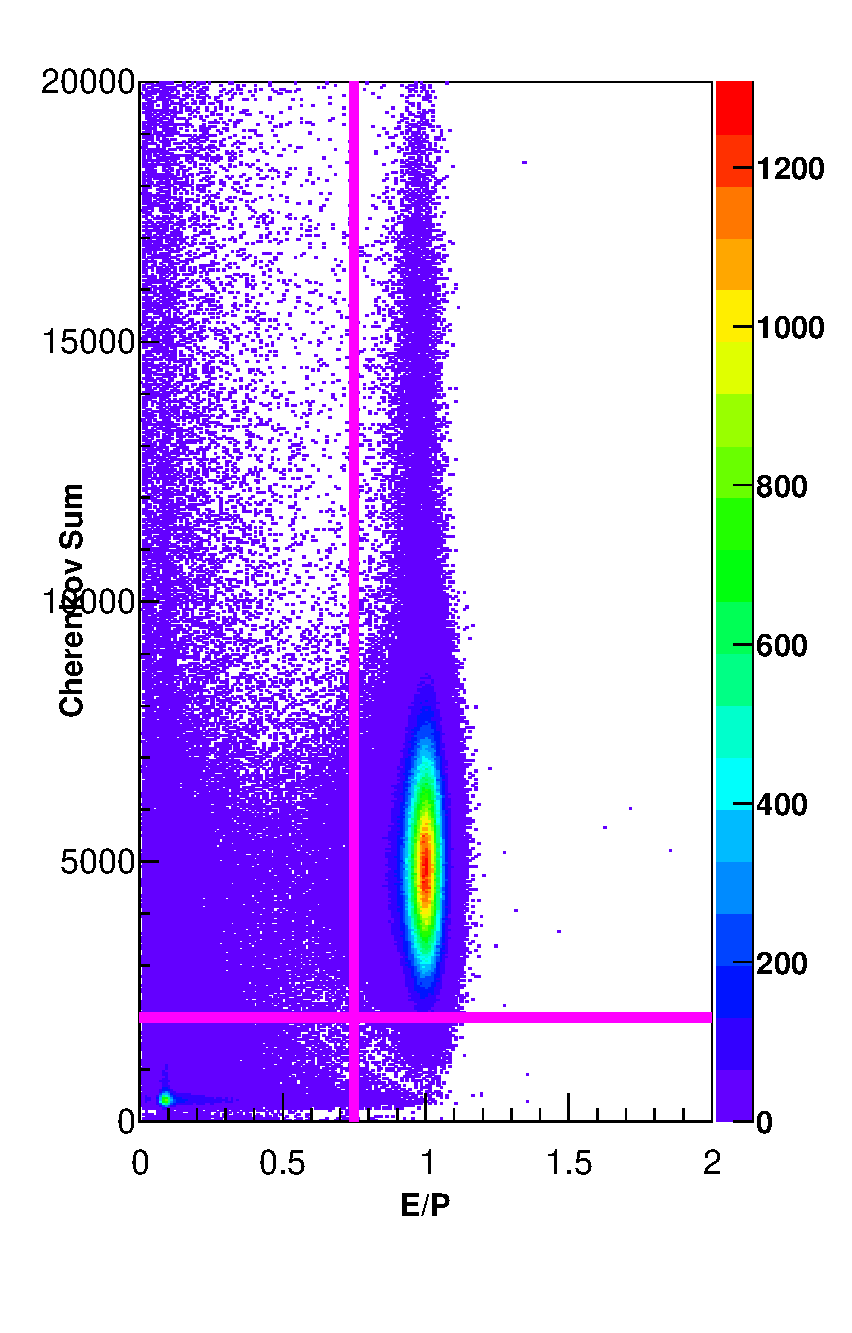
\includegraphics[width=2in]{./pid_plot/pid1.eps}
\end{minipage}
}\\
\centering
\subfigure[kin15]{
\begin{minipage}[t]{1\linewidth}
\centering
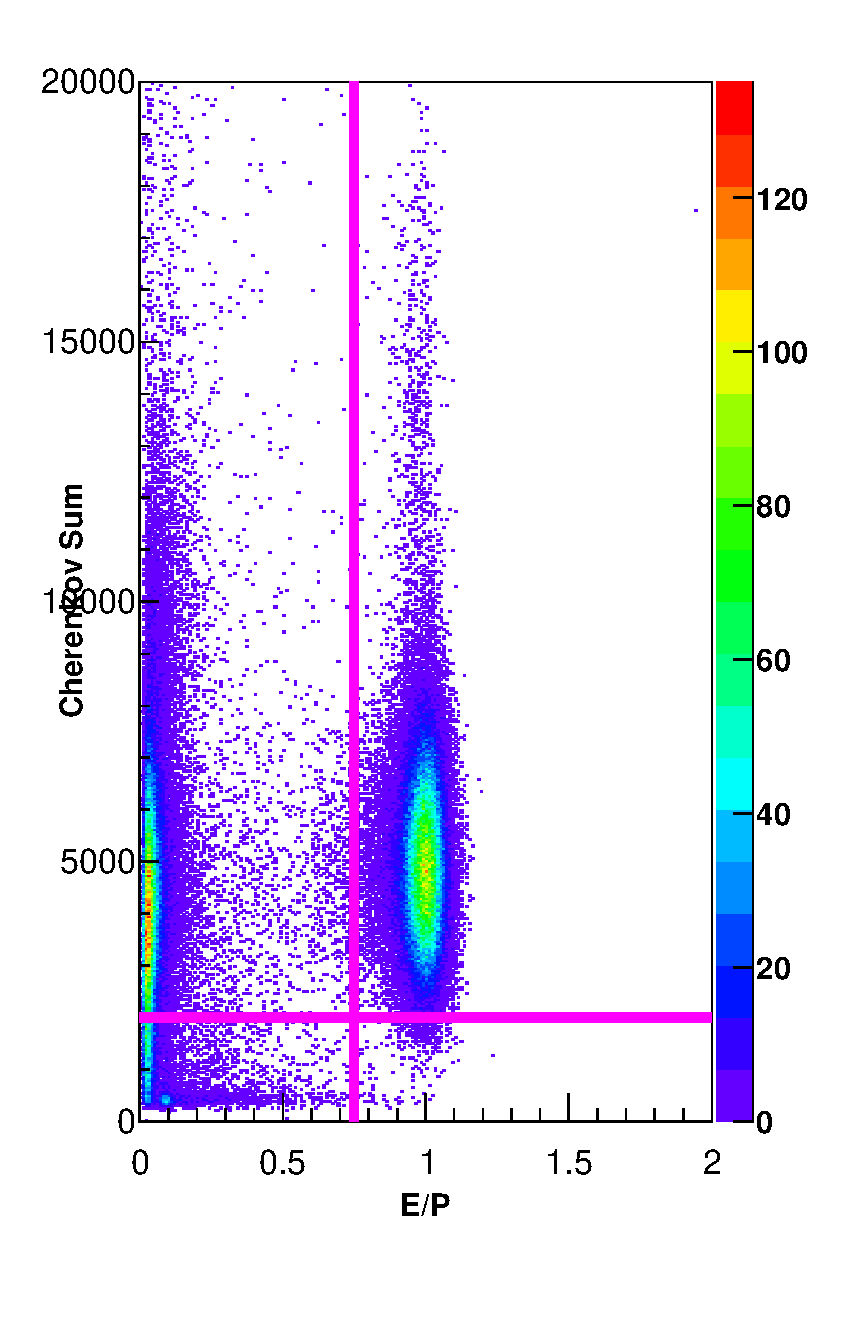
\includegraphics[width=2in]{./pid_plot/pid2.eps}
\end{minipage}
}
\centering
\caption{The 2 PID detector performance for $^{3}H$ at two differnet kinematics setting. General acceptance cut, T2 trigger cut, single track cut and a postive beta cut applied. The two magenta lines indicate the two cut postions for the Cherenkov(horizontal,2000) and E/P(vertical 0.7).  As we can see, different kinematics the ratio of X1 and X2 are different}
\label{pid1}
\end{figure}
The possible explanations for these suspicious signals including 1) for 11 GeV scattering, the high energy neutral particles hitting the back of the HRS dipole and getting into the acceptance and 2) the muon from $\pi^{0}$ decay can have chance to get into the acceptance and have chance to introduce big signal in the Cherenkov. To identify what exactly these signals are still need some work but because of the existence of these signals, there will be a challenge to use the traditional way to check the PID cut efficiency since the as shown in the Table \ref{sample1}, almost no clean sample can be selected out. 
\begin{table}[!ht]
\large
\centering
 \caption{Possibility to cut a pure sample from individual PID detectors}\label{tab:tablenotes}
\begin{threeparttable}
\begin{tabular}[t]{|c|c|c|}\hline
  Experimental Settings & Cherenkov & Calorimeter  \\ \hline        
  electron          &   $\times$ & $\surd$ \\ \hline
  X1                 &  $\times$  & difficult \\  \hline
 X2                  & $\times$  &   difficult\\  \hline  

 \end{tabular}
\begin{tablenotes}
\centering
        \item[1]  $ \times $ means "No", $ \surd $ means "Yes"
 \end{tablenotes}
\end{threeparttable}
\label{sample1} 
 \end{table}
\section{A compromised solution for the PID efficiency check}
Despite that more than one kind of the signals can fire gas Cherenkov and three peaks can be introduced in the calorimeter, if only electrons signals are taken care, we can treat the two calorimeter insensitive signals as a whole non-electron signals and define the four efficiency  in the Table \ref{eff1} 

\begin{table}[!ht]
\large
\centering
 \caption{efficiency defination for the 2 PID detectors}\label{tab:tablenotes}
\begin{tabular}[t]{|c|c|}\hline
   
  $P_{a}^{x}$          &   non-electrons efficiency for Cherenkov \\ \hline
  $P_{a}^{e}$                  &  electrons efficiency for Cherenkov \\  \hline
  $P_{b}^{x}$                 & non-electrons efficiency for Calrimator \\  \hline  
  $P_{b}^{e}$          &    electron efficiency for Calrimator \\  \hline

 \end{tabular}
 \label{eff1}
 \end{table}

After treating all the non-electrons signals as a whole, a clean sample of electron (or non-electron) can be selected form the calorimeter(Table \ref{sample2} and Fig \ref{sample3})
\begin{table}[!ht]
\large
\centering
 \caption{Possibility to cut a pure sample from individual PID detectors}\label{tab:tablenotes}
\begin{threeparttable}
\begin{tabular}[t]{|c|c|c|}\hline
  Experimental Settings & Cherenkov & Calorimeter  \\ \hline        
  electron          &   $\times$ & $\surd$ \\ \hline
  non-electron                &  $\times$  & $\surd$ \\  \hline
 \end{tabular}
\begin{tablenotes}
\centering
        \item[1]  $ \times $ means cannot, $ \surd $ means can
 \end{tablenotes}
\end{threeparttable}
\label{sample2}
 \end{table}
 
\begin{figure}
 	\begin{center}
 		\includegraphics[width=0.4\textwidth] {./pid_plot/PID3.png}
 		\caption{electron and non-electron selecting from the calorimeter } \label{sample3}
 	\end{center}
\end{figure}   
 
 
then according the traditional way to check PID efficiency, the $P_{a}^{x}$ and $P_{a}^{e}$ can be calculable base on the Eq \ref{pid_eq1}. Since Cherenkov should behave stable for electron so the $P_{a}^{e}$ should be very close to 1 and its fluctuation should be very small by different kinematic settings. $P_{a}^{x}$ by contrast, is an effective efficiency for two different kinds signals which can be varied by different kinematic settings because of the different rations of X1 and X2 . Utilizing the independence of the two detectors and the following four functions

\begin{equation}  
\left\{  
             \begin{array}{lr}  
             N_{e}+N_{x}=N_{0} \\  
             P_{a}^{e} N_{e}+ P_{a}^{x} N_{x}=N_{1} \\    
             P_{b}^{e} N_{e}+ P_{b}^{x} N_{x}=N_{2} \\     
             P_{a}^{e} P_{b}^{e} N_{e}+ P_{a}^{x} P_{b}^{x} N_{x}=N_{3}\\  
             \end{array}  
\right.  
\label{PID_eq2}
\end{equation}  

The $P_{b}^{e}$,$P_{b}^{x}$,$N_{x}$,$N_{e}$ can be solved. Where the $N_{0}$ is the event number with the following general cut
\begin{equation}  \label{pid_eq3}
\left\{  
             \begin{array}{lr}  
             No \quad of \quad Track ==1 \\  
             -60\quad mrad< \theta_{tg} <60 \quad mrad \\    
             -30\quad mrad<\varphi_{tg} <30\quad  mrad  \\     
             -0.04<dp<0.04\\
             \beta>0  \\
             T2 \quad trigger\quad only
             \end{array}  
\right.  
\end{equation}  
$N_{1}(N_{2})$is the event number with just  additional Cherenkov (E/P) cut  and $N_{3}$ is the event number with two pid detector cut. $N_{x}(N_{e}) $ is the number of non-electrons(electrons) totally in our data after the previous cut. 

The following four plots(Fig \ref{PPID3} and Fig \ref{PPID4}) shows the four efficiencies defined previous for the two PID detectors, and as we can see three of them ($P_{b}^{e}$,$P_{b}^{x}$,$P_{a}^{e}$) are behaved stable for different kinematics and the $P_{a}^{x}$ varies as what we expected.
\begin{figure}[htpb]

\subfigure[electron effciency for Cherenkov]{
\begin{minipage}[t]{1\linewidth}

\includegraphics[width=3in]{./pid_plot/PIDD1.png}
\end{minipage}
}
\subfigure[non-electron effciency for Cherenkov]{
\begin{minipage}[t]{1\linewidth}

\includegraphics[width=3in]{./pid_plot/PIDD2.png}
\end{minipage}
}

\caption{The two PID efficiency for Chenerkov with different kinematic settings (Blue: He3 and Red: H3)  }  \label{PPID3}
\end{figure}

\begin{figure}[htpb] 
\subfigure[electron effciency for calorimeter ]{
\begin{minipage}[t]{1\linewidth}

\includegraphics[width=3in]{./pid_plot/PIDD3.png}
\end{minipage}
}
\subfigure[electron effciency for calorimeter]{
\begin{minipage}[t]{1\linewidth}

\includegraphics[width=3in]{./pid_plot/PID4.png}
\end{minipage}
}

\caption{The two PID efficiency for calorimeter with different kinematic settings  (Blue: He3 and Red: H3)  } \label{PPID4}
\end{figure}



 Since we only analysis electrons, for a certain PID cuts, we cares more about the non-electron contamination. Define 
\begin{equation}  
\left\{   \begin{array}{lr} 
             N_{e}^{TRUE}= P_{a}^{e} P_{b}^{e} N_{e}\\
             N_{e}^{FALSE}= P_{a}^{x} P_{b}^{x} N_{x}
             \end{array}  
\right.  
\end{equation}  
Where the $N_{e}^{FALSE}$ is the non-electron can pass our two PID cuts and $N_{e}^{TRUE}$ is the number of electrons can pass the same cuts, then the non-electron contamination can be calculated by the following 
\begin{equation}\label{eq:eff1}
\dfrac{x}{e}=\dfrac{N_{e}^{FALSE}}{N_{e}^{TRUE}+N_{e}^{FALSE}}
\end{equation}
Fig \ref{PPID5} shows the non-electron contamination at different kinematics settings, as we can see, this contamination is at 10-3 to 10-4 level (even smaller if only cross-section ratio be focused).                                                               
 
\begin{figure}
 	
 		\includegraphics[width=0.5\textwidth]{./pid_plot/PID5.png}
 		\caption{ Non-electron contimination for H3(Red) and He3(Blue) with different kinematic setting  } \label{PPID5}
 	
\end{figure}   
 
%\bibliographystyle{plain}
%\bibliography{ref}


